\documentclass[tikz, border=20pt]{standalone}
\usepackage{tikz}
\usetikzlibrary{arrows.meta,calc,decorations.pathreplacing}

\tikzset{
  pics/feature/.style  args={#1/#2/#3/#4/#5/#6/#7}{% #1=depth, #2=height, #3=width
    code = {
      \coordinate (-out) at (#1/2, 0, 0);
      \coordinate (-in) at (-#1/2, 0, 0);
      \coordinate (A) at (-#1/2, -#2/2, #3/2);
      \coordinate (B) at (#1/2, -#2/2, #3/2);
      \coordinate (C) at (#1/2, #2/2, #3/2);
      \coordinate (D) at (-#1/2, #2/2, #3/2);
      \coordinate (E) at (#1/2, -#2/2, -#3/2);
      \coordinate (F) at (#1/2, #2/2, -#3/2);
      \coordinate (G) at (-#1/2, #2/2, -#3/2);
      \coordinate (H) at (-#1/2, -#2/2, -#3/2);
      \draw [dashed] (H) -- (A);
      \draw [dashed] (H) -- (E);
      \draw [dashed] (H) -- (G);
      % Front face
      \path[draw] (A) -- (B) -- (C) -- (D) -- (A);
      % Right face
      \path[draw] (B) -- (E) -- (F) -- (C) -- (B);
      % Top face
      \path[draw] (F) -- (G) -- (D) -- (C) -- (F);
      \path [draw, decoration={brace,mirror,raise=5pt},decorate](A) -- node[midway, below=6pt]{\scriptsize #4} (B);
      \path [draw, decoration={brace,mirror,raise=5pt},decorate] (B) -- node[midway, right=12pt, below]{\scriptsize #5} (E);
      \path [draw, decoration={brace,mirror,raise=5pt},decorate](E) -- node[midway, right=6pt]{\scriptsize #6} (F);
      \path (F) -- node[midway,above]{\textsf #7}(G);
      \node{\tikzpictext};
}}}

\tikzset{
  pics/dense/.style args={#1/#2/#3/#4}{
    code = {
      \coordinate (-in) at (-#1/2,0);
      \coordinate (-out) at (#1/2,0);
      \draw (-#1/2, -#2/2) -- (#1/2, -#2/2) -- (#1/2, #2/2) -- (-#1/2, #2/2) -- (-#1/2, -#2/2);
      \draw (0, -#2/2) node[below]{\scriptsize #3};
      \path (#1/2, #2/2) -- node[midway,above]{\textsf #4}(-#1/2, #2/2);
}}}

\tikzset{
  pics/conv/.style args={#1/#2/#3}{
    code = {
      \draw [dashed] (0, -#1/2, -#2/2) -- (#3);
      \draw [dashed] (0, -#1/2, #2/2) -- (#3);
      \draw [dashed] (0, #1/2, #2/2) -- (#3);
      \draw [dashed] (0, #1/2, -#2/2) -- (#3);
      \draw (0, -#1/2, -#2/2) -- (0, -#1/2, #2/2) -- (0, #1/2, #2/2) -- (0, #1/2, -#2/2) -- (0, -#1/2, -#2/2);
      \draw (0, 0, #2/2) node[left]{\scriptsize 3};
      \draw (0, #1/2, 0) node[above]{\scriptsize 3};

    }
  }
}

\begin{document}
\tikzstyle{box} = [draw, rectangle, rounded corners, color=black!80, fill=gray!20!blue!10, minimum width=7em, minimum height=3.5em]
\tikzstyle{line>} = [-{Latex[length=2mm]}, color=black!80]
\tikzstyle{<line} = [{Latex[length=2mm]}-, color=black!80]




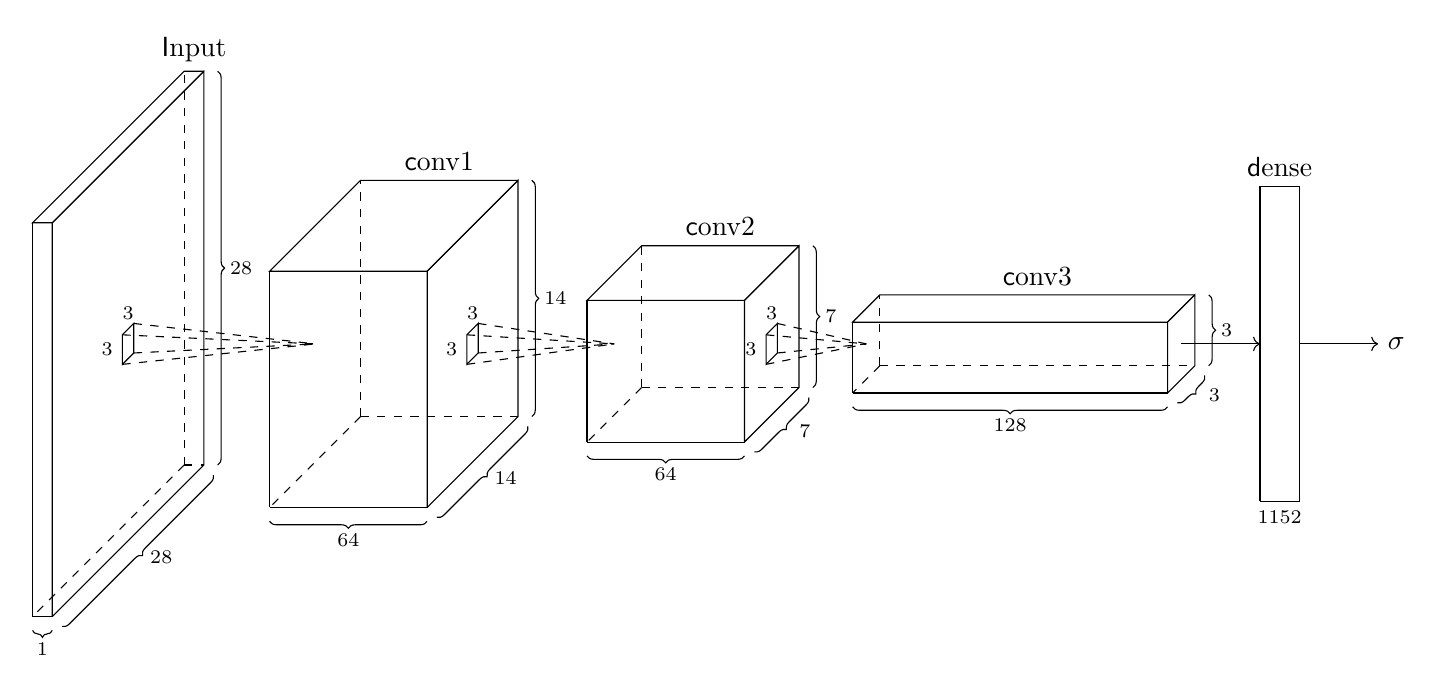
\begin{tikzpicture}
  % \draw (1, 0) pic{dense={0.5/7/768}};
  \pic (feature1) at (2.5, 0) {feature=0.25/5/5/1/28/28/Input};
  \pic (feature2) at (6, 0) {feature={2/3/3/64/14/14/conv1}};
  \pic (feature3) at (9.8, 0) {feature={2/1.8/1.8/64/7/7/conv2}};
  \pic (feature4) at (14, 0) {feature={4/0.9/0.9/128/3/3/conv3}};
  \pic (dense) at (17.25, 0) {dense={0.5/4/1152/dense}};
  \draw (feature1-out) pic[scale=0.5]{conv={0.75/0.75/feature2-in}};
  \draw (feature2-out) pic[scale=0.5]{conv={0.75/0.75/feature3-in}};
  \draw (feature3-out) pic[scale=0.5]{conv={0.75/0.75/feature4-in}};
  \draw [->] (feature4-out) -- (dense-in);
  \draw [->] (dense-out) -- ++(1,0) node[right]{$\sigma$};
  %\pic (conv1) at (feature1-out) {conv={0.75/0.75/feature2-in}};
  % \pic (conv1) at (feature1-out) {conv={0.75/0.75/feature2-in}};
  %\draw (3.125, 0) pic{conv={0.75/0.75}};
  % \draw (5.75, 0) pic[color=black]{features={1.25/4/4}};
  %\draw [->] (features2-out) -- (3, 4);
  %\draw (8.375, 0) pic[color=black]{features={2/1.25/1.25}};
  %\draw (feature2-out) pic[scale=0.5]{conv={0.75/0.75/feature3-in}};
  %\draw (9.375, 0) pic[scale=0.5]{conv={0.5/0.5}};
  % \draw (12.375, 0) pic[color=black]{features={4/0.75/0.75}};

\end{tikzpicture}

\end{document}
